\chapter{Geometrical Combinatorics}
I will not write an introduction here as my thoughts differ on both the sections.\\
While geometrical counting is a sticker to make simple questions feel difficult, geometrical probability is a very powerful technique which is used in research as well.\\
However, I have decided to cover them in the same chapter as they both start with the prefix 'geometric'.\\
\section{Geometric Counting}
\begin{example}
    [Motivating Example]
    How many rectangles of any and all sizes can be formed in a rectangular grid of size $m*n$?
\end{example}
\begin{proof}
    [Solution]
    This can simply be solved by saying that a rectangle is formed when we choose two vertical and two horizontal lines.\\
    In an $m*n$ grid, we have $m+1$ verticals and $n+1$ horizontals. \\
    Hence, we can say the number of rectangles is: $\binom{m+1}{2}*\binom{n+1}{2}$
\end{proof}
This is all geometric counting is. We have a geometric figure and have to count something about it. It is the cheapest trick in the question writers tool box, if a question seems too simple, stick it on the top of a geometric figure and suddenly half the test takers will not attempt it.\\
We don't want to be those people.\\
\section{Geometric Probability}
Geometric probability is a way to calculate probability by measuring the number of outcomes geometrically, in terms of length, area, or volume. Why would we do that? Because sometimes, it is easier to solve for the area than the actual probability. We have a chocolate in India called 'Melody' which has a distinct chocolaty and addictive taste. Its tagline was: "Khud khao, khud jaan jao(Try it yourself to find it for yourself)" The same applies to geometric probability. Let's try it out: \\
\begin{example}
    [Motivating Example]
    (AMC 10 2017)Chloe chooses a real number uniformly at random from the interval $[0, 2017]$. Independently, Laurent chooses a real number uniformly at random from the interval $[0, 4034]$. What is the probability that Laurent’s number is greater than Chloe’s number? (Assume they cannot be equal)
\end{example}
\begin{proof}
    [Solution]
    I have not provided a figure to motivate you to draw it.\\
    Let's call Chloe's number as $x$ and Laurent's number as $y$, all their choices can be represented as a rectangle which is $2017$ units on the x axis and $4034$ units on the y axis. \\
    We are looking for cases where Laurent's number is greater than Chloe's, or $y>x$\\
    This is a line from $(0,0)$ to $(2017,2017)$. We can now find the area of the rectangle above this line divided by the total area of the rectangle which will lead to the answer:\\
    $\frac{(2017+4034)*2017/2}{2017*4034}$\\
    $=\frac{2017*1.5}{2017*2}$\\
    $=\frac{3}{4}$
\end{proof}
Geometric probability can be useful when the number of possible outcomes is infinite and we can easily make a diagram to represent the outcomes.\\
Anther common type of question is:\\
\begin{example}
    A coin of radius $r$ is thrown randomly on a floor tiled with squares of side $l$. Two players bet that the coin will land on exactly one or more than one square respectively. What relation should $l$ and $r$ satisfy for the game to be fair? 
\end{example}
\begin{proof}
    [Solution]
    The coin lies inside the square if the center of the coin is at least $r$ distance away from the boundary of the square.\\
    \begin{figure}[h]
        \centering
        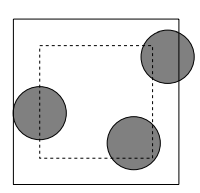
\includegraphics[width=0.5\linewidth]{Photos/Cointoss onto square.png}        
    \end{figure}
    Thus, thus the bet turns to choosing a random point inside a square. If it is at a distance $d\geq r$ then player one wins or else player two wins.\\
    This means for the game to be fair:\\
    $\frac{(l-2r)^2}{l^2}=\frac{1}{2}$\\
    $\iff 2(l-2r)^2=l^2$\\
    $\iff 2l^2-8lr+8r^2=l^2$\\
    $ \iff l^2-8lr+8r^2=0$\\
    This is a quadratic. If you don't know how to solve it, let this question go(or just read the quadratic part from algebra)\\
    $\therefore l=\frac{8r\pm\sqrt{64r^2-32r^2}}{2}$\\
    $\iff l=\frac{8r\pm4r\sqrt{2}}{2}$\\
    $\iff l=4r\pm2r\sqrt{2}$\\
    We reject the minus case as then $l$ will be less than $r$ which is not possible.
    $\therefore l=4r+2r\sqrt{2}$\\
\end{proof}
In conclusion, Geometric probability is the exact converse of geometric counting.There we used to covert a geometrical problem into a counting problem, here we convert a counting problem to a geometry problem. Also it was useless and unnecessary, while this is useful and beautiful.\\
Solve at least questions worth \points{45}. This exercise has a total of \points{60}.
\begin{xcb}{Exercises}
\begin{enumerate}
\item(AMC 10 2004) \points{2} The $5\times 5$ grid shown contains a collection of squares with sizes from $1\times 1$ to $5 \times 5$. How many of these squares contain the black center square?
\begin{center}
    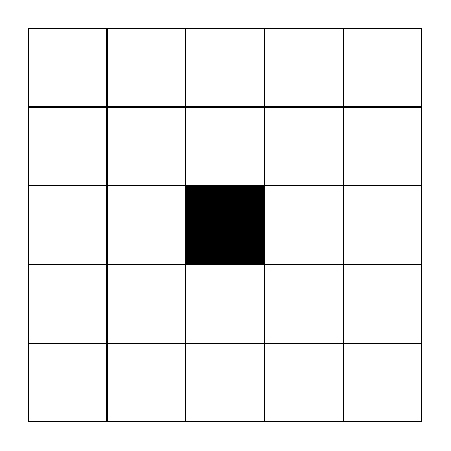
\begin{tikzpicture}
  % Draw outer square
  \draw (0,0) grid (5,5);
  % Draw inner black square
  \fill[black] (2,2) rectangle (3,3);
\end{tikzpicture}
\end{center}
\begin{hint}
    \addhint{Just count!}
\end{hint}
\item(Extension to 1) \points{3} How many rectangles formed by the grid lines in this $5\times 5$ grid contain the black center square?
\item(AMC 10 2007) \points{3} A set of $25$ square blocks is arranged into a $5*5$ square. How many different combinations of $3$ blocks can be selected from that set so that no two are in the same row or column?
\item(AMC 10 2021) \points{3} How many ways are there to place $3$ indistinguishable red chips, $3$ indistinguishable blue chips, and $3$ indistinguishable green chips in the squares of a $3$ by $3$ grid so that no two chips of the same color are directly adjacent to each other, either vertically or horizontally?
\begin{hint}
    \addhint{The cases seem to be less enough that maybe just counting for one colour followed by some multiplication is good sauce.}
\end{hint}
\item (AIME 2006) \points{5} There is an unlimited supply of congruent equilateral triangles made of colored paper. Each triangle is a solid color with the same color on both sides of the paper. A large equilateral triangle is constructed from four of these paper triangles. Two large triangles are considered distinguishable if it is not possible to place one on the other, using translations, rotations, and/or reflections, so that their corresponding small triangles are of the same color. Given that there are six different colors of triangles from which to choose, how many distinguishable large equilateral triangles may be formed?
\begin{hint}
    \addhint{Focus on the color of the center triangle}
    \addhint{Case work onto number of same color triangles on the outside.}
\end{hint}
\item (AMC 10 2019) \points{5} Real numbers between $0$ and $1$, inclusive, are chosen in the following manner. A fair coin is flipped. If it lands heads, then it is flipped again and the chosen number is $0$ if the second flip is heads, and 1 if the second flip is tails. On the other hand, if the first coin flip is tails, then the number is chosen uniformly at random from the closed interval $[0, 1]$. Two random numbers x and y are chosen independently in this manner. What is
the probability that $|x - y| > \frac{1}{2}$?
\begin{hint}
    \addhint{Case work onto the possible coin flips results}
\end{hint}
\item (AIME 2004) \points{3} A circle of radius $1$ is randomly placed in a $15 \times 36$ rectangle ABCD so that the circle lies completely within the rectangle. Given that the probability that the circle will not touch diagonal AC is $m/n$, where m and n are relatively prime positive integers. Find $m + n$.
\item (AIME 1989) \points{2} $10$ points are marked on a circle. How many distinct convex polygons can be made using a subset of them as vertices?
\item \points{3} There are $10$ points on the circumference of a circle. How many points of intersection of line segments with ends at these points will be inside the circle?
\begin{hint}
    \addhint{While some lines will intersect outside, won't every four points give us a pair of two lines intersecting inside?}
\end{hint}
\item \points{2} There are 6 points on the x axis and 9 points on the y axis. How many points of intersection of these points lie in  the first quadrant?
\item \points{2} There are 10 lines in a plane, with no three being concurrent and no two being parallel. How many triangles can be formed using there points of intersection?
\item \points{2} Sheldon is standing at (0,0,0) and can move one unit along either the x, y or z axis. IN how many ways can he walk up to (3,3,3)?
\item \points{9} Choose $n$ points randomly from a circle, What is the probability that all the points are in one semicircle?
\begin{hint}
    \addhint{Choose one point as reference which is one of the diameter points of the semi-circle, we can lie on either side of the diameter.}
    \addhint{We have $n$ possible reference points}
\end{hint}
\item (Amazon Interview) \points{9} A stick is broken in two random places. What are the odds that the three pieces can form the sides of a triangle? 
\begin{hint}
    \addhint{Take the sides as $x,y-x,n-y$ where $n$ is the length of the stick.}
\end{hint}
\item (OMCC 2003) \points{9} A square board with side-length of $8$ cm is divided into $64$ squares with side-length of $1$ cm each. Each square can be painted black or white. Find the total number of ways to color the board so that every square with side-length of $2$ cm formed with $4$ small squares with a common vertex has two black squares and two white squares.
\begin{hint}
    \addhint{Try fixing a column}
    \addhint{If we get a BB or WW in a column, the other is determined uniquely}
\end{hint}
\end{enumerate}
\end{xcb}